\chapter{Resultados}
\label{chap:resultados}

Este capítulo apresenta os resultados das 480 execuções realizadas (4 coletores $\times$ 4 volumes $\times$ 30 repetições), coletadas no ambiente descrito na Seção~\ref{sec:ambiente}. Os resultados são organizados em torno da métrica primária de sobrecarga, o tempo de resposta do observador (RTT UDP), e das métricas secundárias de consumo de recursos (CPU e memória do WAF e do próprio coletor). Todos os valores são apresentados no formato $\bar{x} \pm \text{IC}_{95\%}$, conforme a metodologia descrita no Capítulo~\ref{chap:metodologia}, e foram agregados pelo \texttt{compare.py} a partir das 30 repetições de cada combinação de coletor e volume $N$. Dois intervalos de confiança que não se sobrepõem são tomados como evidência de diferença entre as médias ao nível $\alpha = 0{,}05$. Os mesmos resultados estão disponíveis em um painel interativo\footnote{\url{https://vnf-lab.up.railway.app}}, que permite filtrar por ferramenta e por volume de mensagens.

\section{Tempo de Resposta do Observador}

O tempo de resposta do observador, que mede o tempo de ida e volta da requisição UDP até a entrega das métricas coletadas, constitui a variável dependente primária deste estudo. A Tabela~\ref{tab:rtt} consolida os valores médios para os quatro volumes de mensagens avaliados, e a Figura~\ref{fig:rtt_barras} os representa graficamente.

\begin{table}[htbp]
\centering
\caption{Tempo de resposta médio do observador (RTT UDP, em ms) por volume de mensagens.}
\label{tab:rtt}
\begin{tabular}{lcccc}
\hline
\textbf{Volume ($N$)} & \textbf{eBPF} & \textbf{Sysstat} & \textbf{Prometheus} & \textbf{Docker} \\
\hline
100.000   & $0{,}5331 \pm 0{,}0029$ & $0{,}6137 \pm 0{,}0046$ & $0{,}6225 \pm 0{,}0035$ & $2{,}5789 \pm 0{,}0108$ \\
500.000   & $0{,}4964 \pm 0{,}0032$ & $0{,}5714 \pm 0{,}0026$ & $0{,}5832 \pm 0{,}0042$ & $2{,}5027 \pm 0{,}0099$ \\
1.000.000 & $0{,}4980 \pm 0{,}0023$ & $0{,}5750 \pm 0{,}0042$ & $0{,}5845 \pm 0{,}0028$ & $2{,}4978 \pm 0{,}0107$ \\
2.000.000 & $0{,}4995 \pm 0{,}0024$ & $0{,}5725 \pm 0{,}0024$ & $0{,}5837 \pm 0{,}0021$ & $2{,}5055 \pm 0{,}0080$ \\
\hline
\end{tabular}
\end{table}

\begin{figure}[htbp]
    \centering
    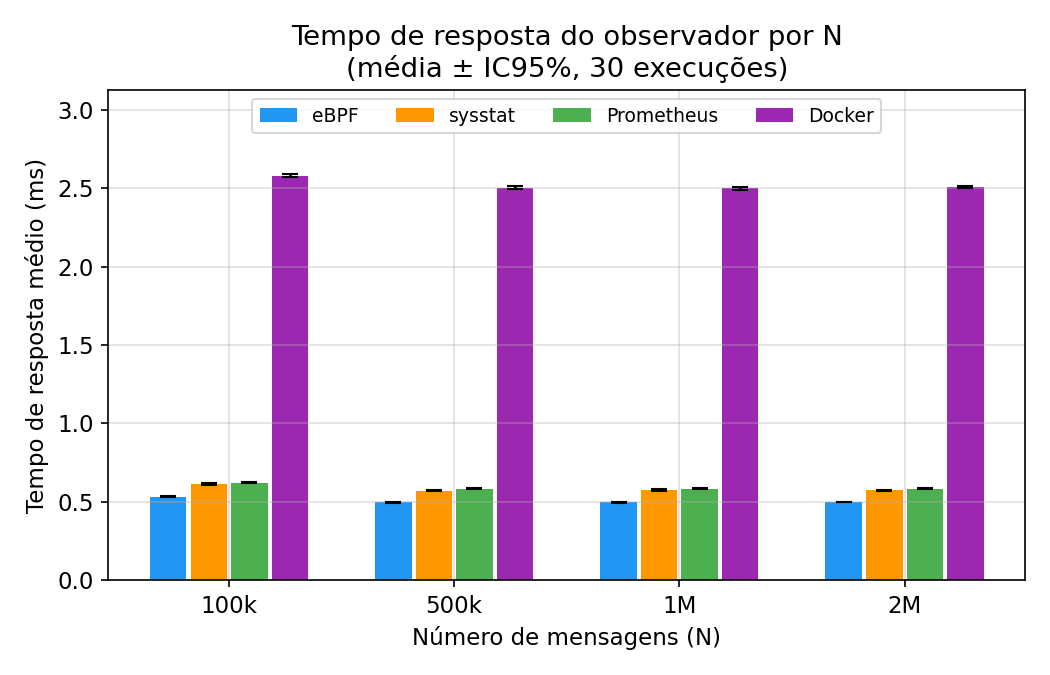
\includegraphics[width=0.85\textwidth]{imagens/tempo_resposta_por_n.png}
    \caption{Tempo de resposta médio do observador por volume de mensagens.}
    \label{fig:rtt_barras}
\end{figure}

O eBPF apresentou o menor tempo de resposta em todos os volumes avaliados. As reduções em relação ao Sysstat variaram de 12,8\% a 13,4\%, e em relação ao Prometheus de 14,4\% a 14,9\%. Em nenhum dos quatro volumes os intervalos de confiança de 95\% do eBPF se sobrepõem aos das demais ferramentas, indicando que a vantagem observada é estatisticamente significativa. Esse comportamento é coerente com a natureza da abordagem: o coletor eBPF lê contadores previamente acumulados em mapas no \textit{kernel}, sem efetuar varreduras de arquivos do \texttt{/proc}, ao passo que os coletores Sysstat e Prometheus realizam, a cada requisição, a leitura e o \textit{parsing} de \texttt{/proc/net/dev} e a consulta a \texttt{psutil} no espaço de usuário.

Entre Sysstat e Prometheus, a diferença é pequena, mas consistente: o Prometheus foi mais lento que o Sysstat em todos os volumes, por 1,4\% a 2,1\%, e os intervalos de confiança não se sobrepõem em nenhum deles. O sentido é compatível com o custo adicional de manter o servidor HTTP ativo, embora a magnitude seja muito inferior à distância que separa ambos do eBPF.

O Docker apresentou o maior tempo de resposta por ampla margem: cerca de $2{,}5$ ms, aproximadamente cinco vezes o do eBPF e pouco mais de quatro vezes o do Sysstat e do Prometheus. A diferença é significativa em todos os volumes. Essa distância é esperada pela estrutura do coletor: ao contrário dos demais, que leem contadores locais, o observador Docker consulta, a cada requisição UDP, o \textit{daemon} do Docker por meio do \textit{socket} Unix, e o \textit{daemon} por sua vez lê os \textit{cgroups} do contêiner e serializa a resposta em JSON. Essa consulta faz parte do caminho medido pelo RTT, de modo que seu custo é integralmente contabilizado. Cabe ressaltar que a decomposição desse tempo entre as etapas da cadeia (observador, \textit{socket}, \textit{daemon}, \textit{cgroup}, serialização) não foi medida neste trabalho; a explicação apresentada é uma hipótese coerente com a arquitetura, e não um resultado experimental. Também não foi avaliada a alternativa de manter a consulta ao \textit{daemon} em segundo plano e responder ao UDP a partir de um valor em \textit{cache}, que reduziria o RTT à custa da atualidade da métrica.

Observa-se também que o tempo de resposta praticamente não varia com o volume de mensagens a partir de $N = 500$ mil, para as quatro ferramentas, com diferenças entre volumes dentro das margens dos intervalos de confiança. A exceção é $N = 100$ mil, que apresenta os maiores tempos médios em todos os coletores (por exemplo, $0{,}5331$ ms no eBPF contra $0{,}4964$ ms em $N = 500$ mil). Uma explicação plausível é a curta duração das execuções de menor volume, em que a fase de inicialização representa fração maior da janela de coleta; essa explicação, contudo, não foi verificada isoladamente.

A Figura~\ref{fig:rtt_boxplot} detalha a distribuição das execuções por meio de diagramas de caixa. Como o tempo do Docker comprime as demais caixas na escala comum, a linha inferior da figura omite essa ferramenta e amplia o eixo. Confirma-se a separação entre as ferramentas: em todos os volumes, as caixas do eBPF, do conjunto Sysstat/Prometheus e do Docker ocupam faixas distintas do eixo, e na visão ampliada a caixa do eBPF situa-se abaixo das do Sysstat e do Prometheus, que por sua vez ficam muito próximas entre si. A dispersão entre execuções é pequena para todas as ferramentas, com desvios-padrão entre as 30 execuções de $0{,}006$ a $0{,}012$ ms no eBPF, no Sysstat e no Prometheus, e de $0{,}021$ a $0{,}029$ ms no Docker, ou seja, cerca de 1\% a 2\% da média em todos os casos.

\begin{figure}[htbp]
    \centering
    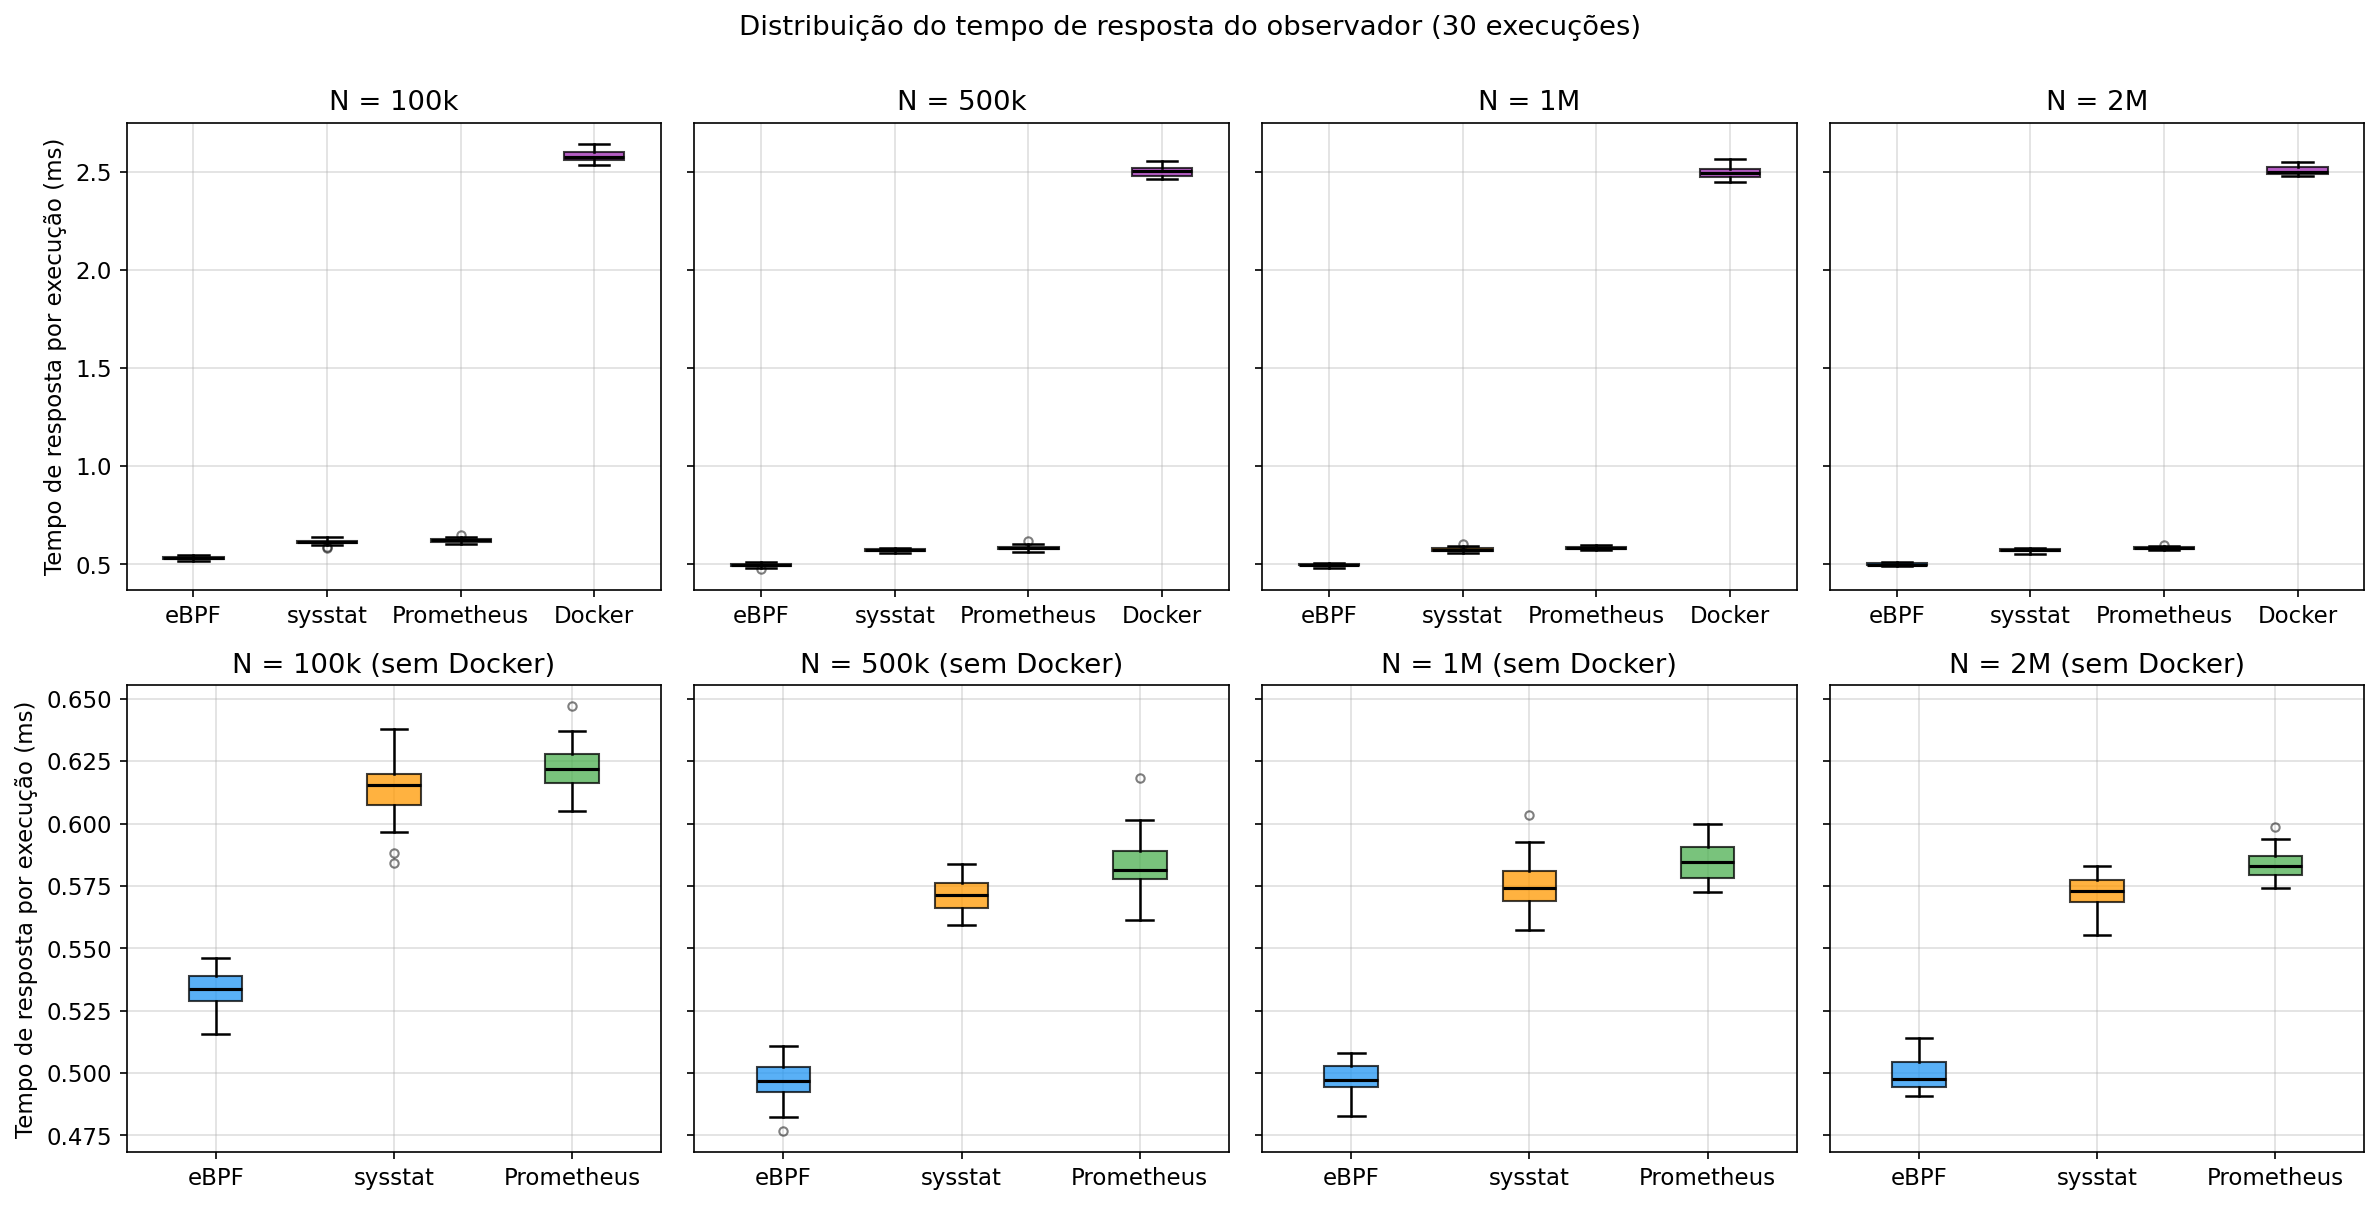
\includegraphics[width=\textwidth]{imagens/boxplot_tempo_resposta.png}
    \caption{Distribuição do tempo de resposta do observador por ferramenta e volume de mensagens (30 execuções). A linha superior mostra as quatro ferramentas; a inferior omite o Docker e amplia o eixo vertical, para tornar visíveis as distribuições do eBPF, do Sysstat e do Prometheus.}
    \label{fig:rtt_boxplot}
\end{figure}

\FloatBarrier
\section{Consumo de CPU do WAF}

O consumo de CPU do processo WAF reflete o custo da inspeção de tráfego, idêntico nos quatro cenários por se tratar da mesma implementação. A Figura~\ref{fig:cpu_waf} mostra que, a partir de $N = 500$ mil, o WAF satura em torno de 104--110\% de uma \textit{thread} (valores superiores a 100\% indicam uso de mais de um núcleo lógico pelo \texttt{ThreadPoolExecutor}), sem diferença prática entre os coletores: em $N = 1$ milhão, por exemplo, os valores são $106{,}09\%$ (eBPF), $105{,}30\%$ (Sysstat), $105{,}30\%$ (Prometheus) e $106{,}05\%$ (Docker).

\begin{figure}[htbp]
    \centering
    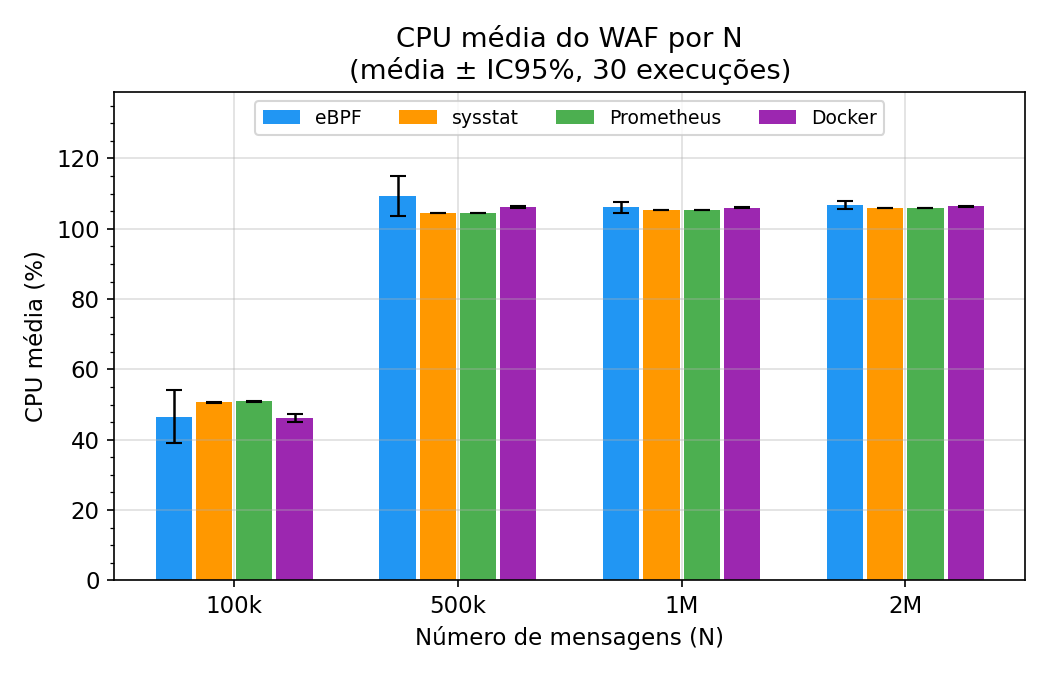
\includegraphics[width=0.85\textwidth]{imagens/cpu_waf.png}
    \caption{Consumo médio de CPU do processo WAF por volume de mensagens.}
    \label{fig:cpu_waf}
\end{figure}

Dois pontos merecem ressalva. Primeiro, em $N = 100$ mil o WAF não chega a operar em regime de saturação (valores de $46\%$ a $51\%$), e o eBPF apresentou intervalo de confiança muito largo ($46{,}48 \pm 7{,}54$), refletindo a grande variabilidade do consumo de CPU em execuções curtas; algo semelhante ocorre com o eBPF em $N = 500$ mil ($109{,}34 \pm 5{,}83$). Dada essa dispersão, não é possível atribuir a diferença ao coletor. Segundo, nos cenários com Docker a CPU do WAF é obtida pela contabilidade do \textit{cgroup}, e não pelo \texttt{psutil} sobre o processo, e os valores ficam ligeiramente acima dos demais em alguns volumes (cerca de $1{,}7\%$ em $N = 500$ mil, com intervalos que não se sobrepõem). Como as duas fontes medem o consumo de maneiras distintas, não se pode afirmar que esse excedente decorra do coletor, e não da diferença de método. Em síntese, o consumo de CPU do WAF é dominado pela carga de inspeção, e os resultados não indicam interferência relevante de nenhum dos coletores sobre ele.

\section{Consumo de Memória}

Esta seção analisa duas memórias distintas, com finalidades diferentes. A memória de interesse comparativo é a do \emph{próprio observador}: ela constitui o \textit{footprint} permanente da ferramenta de monitoramento --- a sobrecarga de memória que o coletor impõe apenas por estar em execução --- e é a dimensão em que as abordagens mais se distinguem, o que justifica seu papel de variável dependente central (cf. Seção~\ref{subsec:requisitos_monitoramento}). A memória do WAF, por sua vez, é reportada como controle: por ser inerente à VNF e decorrer da mesma implementação em todos os cenários, serve para confirmar que a escolha do coletor não altera o consumo da função monitorada.

A Figura~\ref{fig:mem_observador} apresenta o consumo médio de memória do processo observador. O Sysstat consumiu menos ($13{,}6$ MB), seguido do eBPF ($15{,}0$ MB), do Prometheus ($24{,}7$ MB) e do Docker ($30{,}8$ MB). O acréscimo do Prometheus em relação ao Sysstat (cerca de 81\%) decorre diretamente da biblioteca \texttt{prometheus\_client} e do servidor HTTP mantido em execução na porta 8000. O do Docker (cerca de 126\% acima do Sysstat) é compatível com a carga do SDK \texttt{docker} em Python e de suas dependências, mas, como a decomposição não foi medida, trata-se de uma explicação provável, e não verificada.

\begin{figure}[htbp]
    \centering
    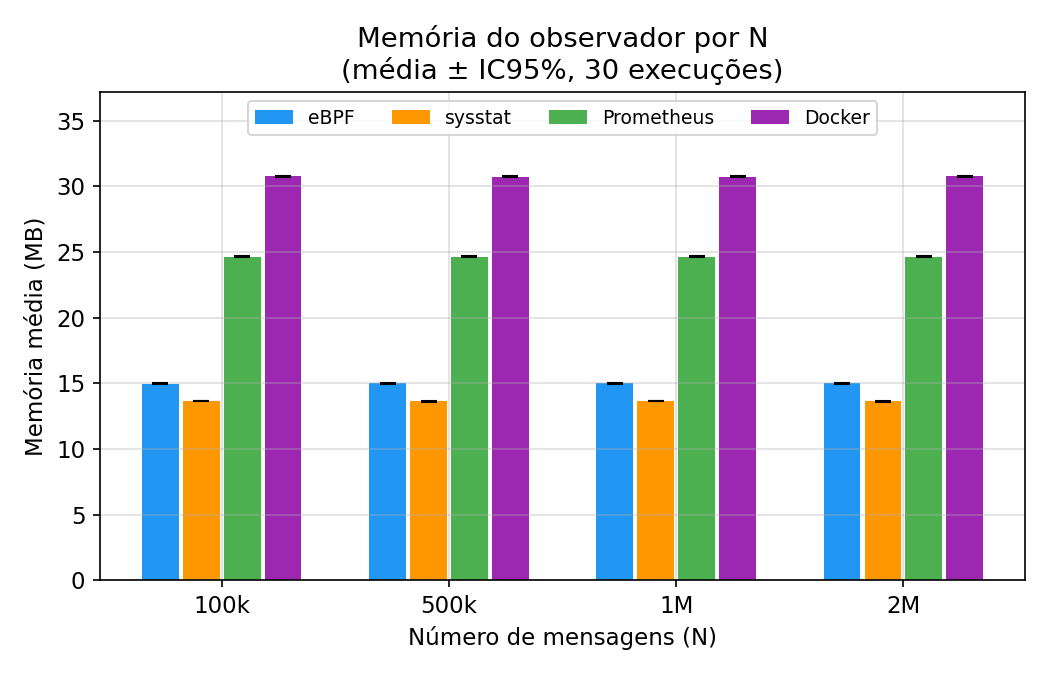
\includegraphics[width=0.85\textwidth]{imagens/memoria_observador.png}
    \caption{Consumo médio de memória do processo observador por volume de mensagens (média $\pm$ IC95\%, 30 execuções).}
    \label{fig:mem_observador}
\end{figure}

O consumo de memória de todos os coletores é praticamente constante ao longo dos quatro volumes de mensagens, com intervalos de confiança estreitos (inferiores a $0{,}06$ MB). Isso confirma que a memória do observador é determinada pela arquitetura de cada ferramenta, e não pelo volume de tráfego processado, comportamento esperado, dado que os coletores mantêm apenas contadores agregados e não armazenam o histórico de mensagens. O eBPF situa-se ligeiramente acima do Sysstat devido ao carregamento do programa BPF e dos mapas no \textit{kernel} pela \textit{libbpf}.

Quanto à memória do próprio WAF, os cenários eBPF, Sysstat e Prometheus apresentaram valores semelhantes, crescendo de cerca de $28$ MB ($N = 100$ mil) para aproximadamente $46$ MB ($N = 2$ milhões), sem diferença atribuível ao coletor. Esse crescimento acompanha o volume de tráfego processado e é inerente à VNF. No cenário Docker, os valores são sistematicamente mais baixos (de $20{,}8$ a $40{,}5$ MB, cerca de $6$ a $8$ MB abaixo dos demais). Essa diferença não deve ser interpretada como economia de memória: no cenário Docker, a memória é a contabilizada pelo \textit{cgroup} (uso total menos o cache de páginas inativo, como no \texttt{docker stats}), enquanto nos demais é o RSS do processo, e as duas métricas medem grandezas distintas. A memória do WAF no cenário Docker não é, portanto, diretamente comparável à dos demais, o que é uma limitação do método de coleta, discutida na Seção~\ref{subsec:coletor_docker}.

\section{Consumo de CPU do Observador}

O consumo de CPU do próprio observador mostrou-se a métrica de medição mais delicada, devido à sua baixa magnitude frente ao ruído de amostragem. As médias dos 16 grupos variam de $0{,}05\%$ a $5{,}1\%$, quase sempre com desvios da ordem da própria média. Apenas três grupos apresentaram valor baixo e estável (eBPF e Prometheus em $N = 500$ mil, com $0{,}05\%$ e $0{,}06\%$, e Sysstat em $N = 100$ mil, com $0{,}06\%$); nos demais, a média é elevada por poucas execuções com picos isolados, como o eBPF em $N = 100$ mil ($2{,}97\% \pm 5{,}97$) e em $N = 1$ milhão ($1{,}62\% \pm 2{,}25$). Como os grupos de valor baixo se distribuem entre ferramentas diferentes e a mesma ferramenta alterna entre valores baixos e altos conforme o volume, o padrão não indica um custo contínuo de nenhum coletor.

Essa instabilidade decorre da granularidade da amostragem via \texttt{psutil} sobre intervalos curtos e da contenção de CPU entre os contêineres que compartilham os mesmos núcleos, conforme apontado nas limitações da metodologia. Por esse motivo, o consumo de CPU do observador é interpretado neste trabalho como evidência qualitativa complementar, e não como base para comparações quantitativas entre as ferramentas. Os dados são compatíveis com a expectativa de que a leitura de contadores diretamente dos mapas do \textit{kernel} seja mais barata em CPU, mas não bastam para afirmá-lo.

\section{Métricas de Validação}

Além das métricas de comparação, registraram-se as métricas de validação descritas na metodologia, cujo objetivo é confirmar que as quatro ferramentas observaram a mesma carga de trabalho, e não discriminar as abordagens. O tempo médio de inspeção por carga convergiu para aproximadamente $0{,}080$ ms nas quatro abordagens (em $N = 1$ milhão, $0{,}0798$ ms no eBPF, $0{,}0797$ ms no Sysstat, $0{,}0796$ ms no Prometheus e $0{,}0798$ ms no Docker), confirmando que o custo unitário de processamento do WAF independe do coletor empregado --- comportamento esperado, dado que nenhuma abordagem interfere no caminho de inspeção das requisições. As métricas de inspeção correspondem à última amostra de cada execução, conforme descrito na Seção~\ref{sec:protocolo}.

Observa-se ainda que a contagem de inspeções registrada ao fim da janela de coleta é inferior a $N$ nos volumes maiores (em média cerca de $706$ mil em $N = 1$ milhão e $1{,}25$ milhão em $N = 2$ milhões), ao passo que em $N = 100$ mil ela coincide com $N$. Esse valor é semelhante entre os coletores (por exemplo, $706.407$ no eBPF e $701.667$ no Docker em $N = 1$ milhão), de modo que a carga efetivamente observada é equivalente entre eles. O motivo de a contagem ficar abaixo de $N$ não foi investigado: é compatível com uma vazão sustentada inferior aos 15.000 mensagens por segundo usados no cálculo da duração da janela (Equação~\ref{eq:duration}), mas essa hipótese não foi verificada, e a premissa de que o cliente conclui o envio de todas as cargas dentro da janela merece ser reavaliada.

Os contadores de bytes RX/TX, por outro lado, não são diretamente comparáveis entre as ferramentas, em razão da diferença no ponto de coleta. O coletor eBPF contabiliza exclusivamente o tráfego do WAF (porta de origem 8080), resultando em valores fortemente assimétricos --- em $N = 1$ milhão, cerca de $623$ MB recebidos contra apenas $9$ MB transmitidos, coerente com requisições volumosas e respostas curtas (\texttt{ALLOWED:OK} ou \texttt{BLOCKED}). Já o Sysstat, o Prometheus e o Docker medem todo o tráfego da interface de \textit{loopback} (no Docker, por meio de \texttt{/proc/net/dev}, já que o WAF utiliza a rede do \textit{host} e as estatísticas de rede do \textit{cgroup} não se aplicam), em que cada byte transmitido é também contabilizado como recebido, produzindo valores simétricos e mais elevados (RX $=$ TX, de aproximadamente $692$ a $704$ MB). Essa diferença é inerente ao escopo de medição de cada abordagem, e não a um erro de contabilização; por isso, os bytes RX/TX são empregados apenas para caracterização, e não como critério de comparação entre as ferramentas.

\section{Síntese dos Resultados}

A Tabela~\ref{tab:sintese} resume o desempenho das quatro abordagens nas dimensões avaliadas. O eBPF foi a ferramenta de menor sobrecarga na métrica primária (tempo de resposta) em todos os volumes, com diferença estatisticamente significativa em relação às demais. O Docker foi a de maior tempo de resposta, cerca de cinco vezes o do eBPF. Na CPU do próprio observador, as diferenças entre as ferramentas não foram conclusivas, devido à alta variabilidade entre as execuções. O Sysstat destacou-se pelo menor consumo de memória, enquanto o Docker apresentou o maior, seguido do Prometheus, em razão do servidor HTTP, sem oferecer vantagem de desempenho no escopo testado, no qual o \textit{endpoint} de métricas permanece disponível, mas não é raspado ativamente.

\begin{table}[htbp]
\centering
\caption{Síntese comparativa das quatro abordagens de monitoramento.}
\label{tab:sintese}
\begin{tabularx}{\textwidth}{lXXXX}
\hline
\textbf{Dimensão} & \textbf{eBPF} & \textbf{Sysstat} & \textbf{Prometheus} & \textbf{Docker} \\
\hline
Tempo de resposta (RTT UDP) & Menor ($\sim$0,50 ms) & Intermediário ($\sim$0,57 ms) & Intermediário ($\sim$0,58 ms) & Maior ($\sim$2,5 ms) \\
CPU do WAF & Equivalente & Equivalente & Equivalente & Equivalente (método de medição distinto) \\
Memória do observador & Intermediária ($\sim$15 MB) & Menor ($\sim$14 MB) & Alta ($\sim$25 MB) & Maior ($\sim$31 MB) \\
CPU do observador & Inconclusiva & Inconclusiva (ruidosa) & Inconclusiva (ruidosa) & Inconclusiva (ruidosa) \\
\hline
\end{tabularx}
\end{table}

Os resultados confirmam a hipótese formulada na introdução: por operar em nível de \textit{kernel}, o eBPF apresenta menor tempo de resposta na coleta de métricas em comparação às abordagens de \textit{polling} em espaço de usuário e à consulta à API do Docker, sem impor sobrecarga adicional ao WAF monitorado. A vantagem do eBPF sobre Sysstat e Prometheus é consistente e estatisticamente significativa, mas de magnitude moderada (cerca de 13\% a 15\%); sobre o Docker, é ampla (cerca de 80\%). Esses fatores devem ser ponderados na escolha da ferramenta em conjunto com os requisitos operacionais de cada cenário, discutidos no Capítulo~\ref{chap:consideracoes_finais}. Os valores do Docker devem ainda ser lidos à luz de duas características do coletor: a consulta ao \textit{daemon} compõe o tempo medido, e as métricas de memória provêm do \textit{cgroup}, não sendo comparáveis às demais.
